%!TEX program = xelatex
%!TEX root = geometria_analitica.tex
%%Usar makeindex -s indexstyle.ist arquivo.idx no terminal para gerar o {\'\i}ndice remissivo agrupado por inicial
%%Ap\'os executar pdflatex arquivo

\chapter{Vetores no Espa\c{c}o} % (fold)
\label{cha:vetores_no_espaco}

Fixemos um ponto $O$ no espa\c{c}o, que ser\'a denominado como \textbf{origem}. Tomemos tr\^es retas duas a duas perpendiculares entre si e concorrentes em $O$, que ser\~ao denominados \textbf{eixos coordenados} e ser\~ao denotados por $Ox$, $Oy$ e $Oz$.
\begin{figure}[!h]
  \centering
  \caption{Sistema de coordenadas tridimensionais}
  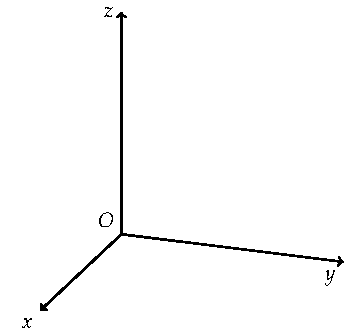
\includegraphics{eixos-coordenados-espaco.pdf}
  % \tdplotsetmaincoords{70}{110}
  % \begin{tikzpicture}[scale=2,tdplot_main_coords]
  %   \coordinate[label=above left:$O$] (A) at (0,0,0);
    
  %   %constr\'oi os eixos cartesianos
  %   \draw[thick,->,black] (0,0,0) -- (2,0,0) node[anchor=north east]{$x$};
  %   \draw[thick,->] (0,0,0) -- (0,2,0) node[anchor=north east]{$y$};
  %   \draw[thick,->] (0,0,0) -- (0,0,2) node[anchor=east]{$z$};
  %   \end{tikzpicture}
\end{figure}

Projetando um ponto $P$ do espa\c{c}o ortogonalmente sobre cada um dos eixos coordenados podemos representar os pontos do espa\c{c}o por ternas ordenadas $(a,b,c)$ de n\'umeros reais.

\begin{figure}[!h]
  \centering
  \caption{Coordenadas de um ponto no espa\c{c}o tridimensional}
  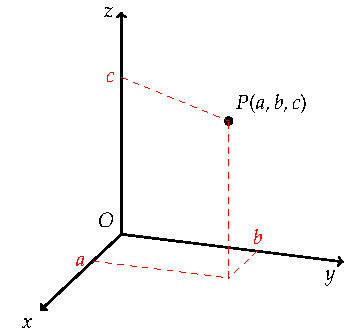
\includegraphics{coordenadas-ponto-espaco.pdf}
  % \tdplotsetmaincoords{70}{110}
  % \begin{tikzpicture}[scale=2,tdplot_main_coords]
  %   \coordinate[label=above left:$O$] (A) at (0,0,0);
    
  %   %constr\'oi os eixos cartesianos
  %   \draw[thick,->,black] (0,0,0) -- (2,0,0) node[anchor=north east]{$x$};
  %   \draw[thick,->] (0,0,0) -- (0,2,0) node[anchor=north east]{$y$};
  %   \draw[thick,->] (0,0,0) -- (0,0,2) node[anchor=east]{$z$};

  %   \tdplotsetcoord{P}{2}{45}{60}
  %   \filldraw (P) circle (1pt) node[above right]{$P(a, b, c)$};

  %   \draw[dashed, color=red] (Px) -- (Pxy) node[at start,left]{$a$};
  %   \draw[dashed, color=red] (Py) -- (Pxy)node[at start,above]{$b$};
  %   \draw[dashed, color=red] (Pz) -- (P)node[at start,left]{$c$};
  %   \draw[dashed, color=red] (Pxy) -- (P);
  %   \end{tikzpicture}
\end{figure}

Assim os pontos de $\real^3$ s\~ao descritos por
\[
  \real^3 = \{(a,b,c)\mid a,b,c \in \real\}.
\]

Sejam $P(x_1,y_1,z_1)$ e $Q(x_2,y_2,z_2)$ dois pontos de $\real^3$. Tra\c{c}ando por $P$ um segmento $PS$ paralelo ao segmento $P_0Q_0$, onde $P_0(x_1,y_1)$ e $Q_0(x_2,y_2)$, obtemos que
\[
  d(P,Q)^2 = d(P_0,Q_0)^2 + |SQ|^2.
\]
\begin{figure}
  \centering
  \caption{Dist\^ancia entre pontos em $\real^3$}
  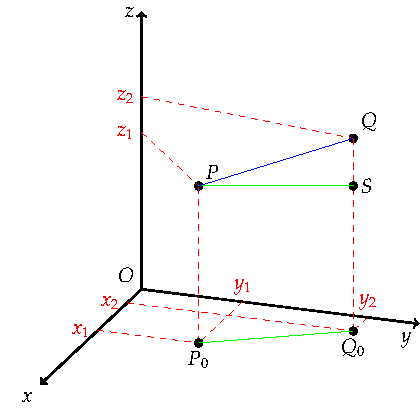
\includegraphics{distancia-pontos-espaco.pdf}
  % \tdplotsetmaincoords{70}{110}
  % \begin{tikzpicture}[scale=2,tdplot_main_coords]
  %   \coordinate[label=above left:$O$] (A) at (0,0,0);
    
  %   %constr\'oi os eixos cartesianos
  %   \draw[thick,->,black] (0,0,0) -- (2.5,0,0) node[anchor=north east]{$x$};
  %   \draw[thick,->] (0,0,0) -- (0,2.5,0) node[anchor=north east]{$y$};
  %   \draw[thick,->] (0,0,0) -- (0,0,2.5) node[anchor=east]{$z$};

  %   \tdplotsetcoord{P}{2}{45}{40}
  %   \filldraw (P) circle (1pt) node[above right]{$P$};
  %   \tdplotsetcoord{Q}{2.7}{50}{80}
  %   \filldraw (Q) circle (1pt) node[above right]{$Q$};

  %   \draw[dashed, color=red] (Px) -- (Pxy) node[at start,left]{$x_1$};
  %   \draw[dashed, color=red] (Py) -- (Pxy)node[at start,above]{$y_1$};
  %   \draw[dashed, color=red] (Pz) -- (P)node[at start,left]{$z_1$};
  %   \draw[dashed, color=red] (Pxy) -- (P);
  %   \draw[dashed, color=red] (Qx) -- (Qxy) node[at start,left]{$x_2$};
  %   \draw[dashed, color=red] (Qy) -- (Qxy)node[at start,above]{$y_2$};
  %   \draw[dashed, color=red] (Qz) -- (Q)node[at start,left]{$z_2$};
  %   \draw[dashed, color=red] (Qxy) -- (Q);

  %   \filldraw ($(Q)!(P)!(Qxy)$) circle (1pt)node[right]{$S$};
  %   \draw[color=green] ($(Q)!(P)!(Qxy)$) -- (P);
  %   \filldraw (Pxy) circle (1pt) node[below]{$P_0$};
  %   \filldraw (Qxy) circle (1pt) node[below]{$Q_0$};

  %   \draw[color=blue] (P) -- (Q);
  %   \draw[color=green] (Pxy) -- (Qxy);
  %   \end{tikzpicture}
\end{figure}

Agora, $|SQ| = |z_2 - z_1|$ e da{\'\i}
\[
  D(P,Q) = \sqrt{(x_1 - x_2)^2 + (y_1 - y_2)^2 + (z_1 - z_2)^2}.
\]

\begin{exemplos}
  A dist\^ancia entre os pontos $P(2,-1,1)$ e $Q(-3,4,2)$ \'e
  \[
    d(P,Q) = \sqrt{[2 - (-3)]^2 + (-1-4)^2 + (1-2)^2} = \sqrt{51}.
  \]
\end{exemplos}

Os vetores e as opera\c{c}\~oes com eles podem ser definidas utilizando-se dos eixos coordenados do espa\c{c}o. Para isso, um ponto $P$ do espa\c{c}o \'e representado em $\real^3$ por uma terna de coordenadas $P(x_1, y_1,z_1)$, onde $x_1$, $y_1$, $z_1 \in \real$.

Seja $\vec{u}$ um vetor no espa\c{c}o. Sabemos que $\vec{u}$ \'e um representante de uma certa classe de equipol\^encia dos segmentos orientados $(B,C)$. Para este segmento orientado $(B,C)$ podemos encontrar um ponto $A(x_1, y_1,z_1)$ tal que o segmento orientado $(O,A)$, onde $O(0,0,0)$, tem o mesmo comprimento, a mesma dire\c{c}\~ao e o mesmo sentido de $(B,C)$. Assim o vetor $\vec{u}$ pode ser representado pelo segmento orientado $(O,A)$. Portanto qualquer vetor em $\real^3$ pode ser representado como um segmento com origem no ponto $(0,0,0)$ e extremidade em um ponto $(x_1,y_1,z_1)$.


Assim escrevemos $\vec{u} = \vec{OP}$. Para simplificar a nota\c{c}\~ao vamos identificar o vetor $\vec{u} = \vec{OP}$ com as coordenadas de sua extremidade e da{\'\i} escrevemos
\[
  \vec{u} = (x_1,y_1,z_1).
\]
As coordenadas $(x_1,y_1,z_1)$ s\~ao chamadas de \textbf{componentes} do vetor $\vec{u}$. Com essa representa\c{c}\~ao, o vetor nulo $\vec{0}$ \'e escrito como
\[
  \vec{0} = (0,0,0).
\]

Desse modo, podemos reescrever a defini\c{c}\~ao de soma e produto por escalar da seguinte forma:
\begin{definicao}
  Sejam $\alpha \in \real$, $\vec{u} = (x_1, y_1,z_1)$ e $\vec{v} = (x_2, y_2,z_2)$. Ent\~ao:
  \begin{enumerate}
    \item $\vec{u} + \vec{v} = (x_1 + x_2, y_1 + y_2,z_1 + z_2)$;
    \item $\alpha \vec{u} = (\alpha x_1, \alpha y_1, \alpha z_1)$.
  \end{enumerate}
\end{definicao}

% \begin{center}
%   \begin{tikzpicture}[scale=2]%soma de vetores no plano
%     \coordinate (A) at (0,0);
%     \coordinate (V) at (0.5,1);
%     \coordinate (W) at (1,0.5);
%     \coordinate (B) at (0,1);
%     \coordinate (VW) at ($(V)+(W)$);
%     %defini\c{c}\~ao das coordenadas dos eixos cartesianos
%     \coordinate (F) at (-1,0);
%     \coordinate (G) at (0,-1);
%     \coordinate (X) at (2,0);
%     \coordinate (Y) at (0,2);
%     % Styles
%     \tikzstyle{axes}=[]

%     \begin{scope}[style=axes]%constr\'oi os eixos cartesianos
%     \draw[->] (F) -- (X) node[below] {$x$} coordinate(x axis);
%     \draw[->] (G) -- (Y) node[left] {$y$} coordinate(y axis);
%     \end{scope}

%     \draw[->,>=triangle 45,color=blue] (A)--(V)
%       node[above]{$\vec{u}$};
%     \draw[->,>=triangle 45,color=blue] (A)--(W)
%       node[below right]{$\vec{v}$};
%     \draw[->,>=triangle 45,color=red] (A)--(VW)
%       node[below right]{$\vec{u}+\vec{v}$};
%     \draw[dashed,>=triangle 45,color=blue] (V)--(VW);
%     \draw[dashed,>=triangle 45,color=blue] (W)--(VW);
%     \draw[dashed,color=black] let \p1 = (V) in (\x1,0) -- (\x1,\y1)
%       node[at start, below]{$x_1$};
%     \draw[dashed,color=black] let \p1 = (V) in (0,\y1) -- (\x1,\y1)
%       node[at start, left]{$y_1$};
%     \draw[dashed,color=black] let \p1 = (W) in (\x1,0) -- (\x1,\y1)
%       node[at start, below]{$x_2$};
%     \draw[dashed,color=black] let \p1 = (W) in (0,\y1) -- (\x1,\y1)
%       node[at start, left]{$y_2$};
%     \draw[dashed,color=black] let \p1 = (VW) in (\x1,0) -- (\x1,\y1)
%       node[at start, below]{$x_1 + x_2$};
%     \draw[dashed,color=black] let \p1 = (VW) in (0,\y1) -- (\x1,\y1)
%       node[at start, left]{$y_1 + y_2$};
%   \end{tikzpicture}

%   \begin{tikzpicture}[scale=2]%multiplica\c{c}\~ao por escalar no plano
%     \coordinate (A) at (0,0);
%     \coordinate (V) at (0.5,0.5);
%     \coordinate (W) at ($2*(V)$);
%     %defini\c{c}\~ao das coordenadas dos eixos cartesianos
%     \coordinate (F) at (-1,0);
%     \coordinate (G) at (0,-1);
%     \coordinate (X) at (2,0);
%     \coordinate (Y) at (0,2);
%     % Styles
%     \tikzstyle{axes}=[]

%     \begin{scope}[style=axes]%constr\'oi os eixos cartesianos
%     \draw[->] (F) -- (X) node[below] {$x$} coordinate(x axis);
%     \draw[->] (G) -- (Y) node[left] {$y$} coordinate(y axis);
%     \end{scope}

%     \draw[->,>=triangle 45,color=blue] (A)--(V)
%       node[above]{$\vec{u}$};
%     \draw[->,>=triangle 45,color=red] (A)--(W)
%       node[below right]{$\alpha \vec{u}$};
%     \draw[dashed,color=black] let \p1 = (V) in (\x1,0) -- (\x1,\y1)
%       node[at start, below]{$x_1$};
%     \draw[dashed,color=black] let \p1 = (V) in (0,\y1) -- (\x1,\y1)
%       node[at start, left]{$y_1$};
%     \draw[dashed,color=black] let \p1 = (W) in (\x1,0) -- (\x1,\y1)
%       node[at start, below]{$\alpha x_1$};
%     \draw[dashed,color=black] let \p1 = (W) in (0,\y1) -- (\x1,\y1)
%       node[at start, left]{$\alpha y_1$};
%   \end{tikzpicture}
% \end{center}

Em alguns casos pode ser mais conveniente representar um vetor $\vec{u} = (x_1, y_1,z_1)$ de forma matricial. Para isso escrevemos as componentes de $\vec{u}$ como uma matriz de 1 coluna e tr\^es linhas
\[
  \vec{u} = \begin{bmatrix}
    x_1\\y_1\\z_1
  \end{bmatrix}.
\]

Vimos que a norma de um vetor \'e definida como o comprimento de um segmento orientado que o represente. Com a representa\c{c}\~ao de vetores por coordenadas podemos reescrever o conceito de norma da seguinte maneira:
\begin{definicao}
  Seja $\vec{u} = (x_1, y_1,z_1)$ um vetor. A \textbf{norma} de $\vec{u}$, denotada por $\norm{\vec{u}}$ \'e dada por
  \[
    \norm{\vec{u}} = \sqrt{x_1^2 + y_1^2 + z_1^2}.
  \]
\end{definicao}

Um vetor de norma 1 \'e chamado de \textbf{vetor unit\'ario}. Dado um vetor n\~ao nulo $\vec{u}$ o vetor
\[
  \vec{v} = \dfrac{\vec{u}}{\norm{\vec{u}}}
\]
\'e um vetor unit\'ario na dire\c{c}\~ao de $\vec{u}$ pois
\[
  \norm{\vec{v}} = \norm{\dfrac{\vec{u}}{\norm{\vec{u}}}} = \dfrac{1}{\norm{\vec{u}}}\norm{\vec{u}} = 1.
\]

\begin{exemplo}
  Seja $\vec{u} = (-2,3,2)$ um vetor. Ent\~ao
  \begin{align*}
    \norm{\vec{u}} &= \sqrt{(-2)^2 + 3^2 + 2^2} = \sqrt{17}\\
    \vec{v} &= \dfrac{\vec{u}}{\norm{u}} = \dfrac{1}{\sqrt{17}}(-2,3,2) = \left(\dfrac{-2}{\sqrt{17}}, \dfrac{3}{\sqrt{17}}, \dfrac{2}{\sqrt{17}}\right).
  \end{align*}
\end{exemplo}
% section vetores_plano (end)

\begin{proposicao}
  Sejam $\vec{u} = (x_1, y_1,z_1)$ um vetor em $\real^3$ e $\alpha \in \real$. Ent\~ao:
  \begin{enumerate}
    \item Se $\vec{u} \ne \vec{0}$, ent\~ao $\norm{\vec{u}} \ne 0$.
    \item $\norm{\vec{u}} \ne 0$ se, e somente se, $\vec{u} \ne \vec{0}$.
    \item $\norm{\alpha\vec{u}} = |\alpha|\norm{\vec{u}}$.
  \end{enumerate}
\end{proposicao}
\begin{prova}
  \begin{enumerate}
    \item  Se $\vec{u} \ne (0,0,0) = \vec{0}$, ent\~ao $x_1 \ne 0$ ou $y_1 \ne 0$ ou $z_1 \ne 0$. Da{\'\i}
    \[
      \norm{\vec{u}} = \sqrt{x_1^2 + y_1^2 + z_1^2} > 0.
    \]
    \item $\norm{\vec{u}} = 0$ se, e somente se, $x_1^2 + y_1^2 + z_1^2 = 0$, isto \'e, $x_1 = y_1 = z_1 = 0$. Portanto $\vec{u} = \vec{0}$.
    \item $\norm{\alpha\vec{u}} = \norm{\alpha(x_1, y_1, \alpha z_1)} = \sqrt{(\alpha x_1)^2 + (\alpha y_1)^2 + (\alpha z_1)^2} = \sqrt{\alpha^2(x_1^2 + y_1^2 + z_1^2)} = |\alpha|\norm{\vec{u}}$.
  \end{enumerate}
\end{prova}

\subsection{\^Angulo entre vetores e produto interno no espa\c{c}o} % (fold)
\label{sub:angulo_entre_vetores_e_produto_interno_no_espaco}
\begin{definicao}
  Sejam $\vec{u}$ e $\vec{v}$ vetores n\~ao nulos. O \textbf{\^angulo} entre $\vec{u}$ e $\vec{v}$ \'e definido pelo \^angulo $\theta$ determinado por $\vec{u}$ e $\vec{v}$ e que satisfaz $0 \le \theta \le \pi$, quando os vetores $\vec{u}$ e $\vec{v}$ s\~ao representados com a mesma origem.\index{Vetores!\^Angulo}
\end{definicao}

\begin{definicao}
  Quando o \^angulo $\theta$ entre dois vetores $\vec{u}$ e $\vec{v}$ \'e reto, isto \'e, $\theta = \pi/2$, ou um deles \'e o vetor nulo, dizemos que os vetores $\vec{u}$ e $\vec{v}$ s\~ao \textbf{ortogonais} ou \textbf{perpendiculares} entre si. Denotamos tal fato, escrevendo $\vec{u} \perp \vec{v}$.\index{Vetores!Ortogonais}
\end{definicao}

Sejam $\vec{u}$ e $\vec{v}$ vetores n\~ao nulos e $\theta$ o \^angulo entre eles.
\begin{figure}[!h]
  \centering
  \caption{\^Angulo entre vetores em $\real^3$}
  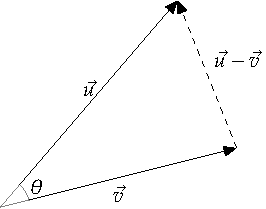
\includegraphics{angulo-vetores-espaco.pdf}
  % \begin{tikzpicture}
  %   \coordinate (A) at (0,0);
  %   \coordinate (X) at (4,1);
  %   \coordinate (Y) at (3,3.5);

  %   \draw[->,>=triangle 45] (A) -- (X)
  %   node[midway,below]{$\vec{v}$};
  %   \draw[->,>=triangle 45] (A) -- (Y)
  %   node[midway,above]{$\vec{u}$};
  %   \draw[dashed,->,>=triangle 45] (X) -- (Y)
  %   node[midway,above right]{$\vec{u} - \vec{v}$};

  %   % Mark the angle XAY
  %   \begin{scope}
  %     \path[clip] (A) -- (X) -- (Y);
  %     \fill[white, opacity=0.5, draw=black] (A) circle (5mm);
  %     \node at ($(A)+(30:7mm)$) {$\theta$};
  %   \end{scope}
  % \end{tikzpicture}
\end{figure}


\begin{definicao}\label{produtointerno-espaco}
  O \textbf{produto escalar} ou \textbf{produto interno} dos vetores $\vec{u}$ e $\vec{v}$, indicado por $\inner{u}{v}$, \'e o n\'umero real tal que\index{Vetores!Produto Escalar}
  \begin{enumerate}
    \item Se $\vec{u}$ ou $\vec{v}$ \'e nulo, ent\~ao $\inner{u}{v} = 0$.
    \item Se $\vec{u}$ e $\vec{v}$ n\~ao s\~ao nulos e $\theta$ \'e o \^angulo entre $\vec{u}$ e $\vec{v}$, ent\~ao
    \begin{align}\label{produto-interno-espaco}
      \inner{u}{v} = \norm{\vec{u}}\norm{\vec{v}}\cos\theta.
    \end{align}
  \end{enumerate}
\end{definicao}

\begin{proposicao}
  Sejam $\vec{u}$ e $\vec{v}$ vetores e $\theta$ o \^angulo entre $\vec{u}$ e $\vec{v}$.
  \begin{enumerate}
    \item Se $\vec{u}$ e $\vec{v}$ n\~ao s\~ao nulos, ent\~ao
    \[
      \cos\theta = \dfrac{\inner{u}{v}}{\norm{\vec{u}}\norm{\vec{v}}}.
    \]
    \item Qualquer que seja o vetor $\vec{u}$,
    \[
      \norm{\vec{u}} = \sqrt{\inner{u}{u}}.
    \]
    \item Quaisquer que sejam os vetores $\vec{u}$ e $\vec{v}$, $\vec{u}\perp\vec{v}$ se, e somente se, $\inner{u}{v} = 0$.
    \end{enumerate}
\end{proposicao}
De modo an\'alogo ao caso para vetores no plano, temos:
\begin{teorema}
  O produto interno de dois vetores $\vec{u} = (x_1, y_1,z_1)$ e $\vec{v} = (x_2, y_2,z_2)$ em $\real^3$ \'e dado por
  \[
    \inner{u}{v} = x_1x_2 + y_1y_2 + z_1z_2.
  \]
\end{teorema}

\begin{exemplos}
  \begin{enumerate}
    \item Sejam $\vec{u} = (2, -3, 1)$ e $\vec{v} = (1,1, 0)$. Determine o \^angulo entre $\vec{u}$ e $\vec{v}$.
    \begin{solucao}
      Temos
      \begin{align*}
        \inner{u}{v} = \langle(2, -3, 1), (1,1,0)\rangle = 2 - 3 + 0 = -1\\
        \norm{\vec{u}} = \sqrt{14},\ \norm{\vec{v}} = \sqrt{2}\\
        \cos\theta = \frac{\inner{u}{v}}{\norm{\vec{u}}\norm{\vec{v}}} = -\dfrac{1}{\sqrt{14}\sqrt{2}} = -\dfrac{1}{\sqrt{28}}.
      \end{align*}
      Assim, $\theta = \arccos\left(-\dfrac{1}{\sqrt{28}}\right)$.
    \end{solucao}
    \item Encontre um vetor $\vec{u} = (x, y, z)$ ortogonal a $\vec{v} = (4, -1, 2)$ e tal que $\inner{u}{w} = -1$, onde $\vec{w} = (1,1,-1)$.
    \begin{solucao}
      Como $\inner{u}{v} = 0$ e $\inner{u}{w} = -1$ obtemos o sistema
      \[
        \begin{cases}
          4x - y + 2z = 0\\
          x + y - z = -1
        \end{cases}
      \]
      cuja solu\c{c}\~ao \'e $x = -1/5 - z/5$ e $y = -4/5 + 6z/5$. Fazendo $z = 0$, obtemos $\vec{u} = (-1/5, -4/5, 0)$.
    \end{solucao}
  \end{enumerate}
\end{exemplos}

\begin{proposicao}\label{propriedades-produto-vetorial-espaco}
  Quaisquer que sejam os vetores $\vec{u} = (x_1, y_1,z_1)$, $\vec{v} = (x_2, y_2,z_2)$ e $\vec{w} = (x_3, y_3,z_3)$ e qualquer que seja o n\'umero real $\lambda$ temos
  \begin{enumerate}[label=({\roman*})]
    \item\label{linearidade-soma-produto-vetorial-espaco} $\langle\vec{u}, (\vec{v} + \vec{w})\rangle = \inner{u}{v} + \inner{u}{w}$
    \item\label{linearidade-escalar-produto-vetorial-espaco} $\langle\vec{u}, (\lambda\vec{v})\rangle = \langle(\lambda\vec{u}), \vec{v}\rangle = \lambda\inner{u}{v}$
    \item $\inner{u}{v} = \inner{v}{u}$
    \item Se $\vec{u} \ne \vec{0}$, ent\~ao $\inner{u}{u} > 0$.
  \end{enumerate}
\end{proposicao}
\begin{prova}
  \begin{enumerate}[label=({\roman*})]
    \item \begin{align*}
      \langle\vec{u}, (\vec{v} + \vec{w})\rangle &= \langle\vec{u}, (x_2 + x_3, y_2 + y_3, z_2 + z_3)\rangle = x_1(x_2 + x_3) + y_1(y_2 + y_3) + z_1(z_2+z_3) \\ &= (x_1x_2 + y_1y_2 + z_1z_2) + (x_1x_3 + y_1y_3 + z_1z_3) = \inner{u}{v} + \inner{u}{w}
    \end{align*}
    \item \begin{align*}
      \langle\vec{u}, (\lambda\vec{v})\rangle &= \langle\vec{u}, (\lambda x_2, \lambda y_2, \lambda z_2)\rangle = x_1(\lambda x_2) + y_1(\lambda y_2) + z_1(\lambda z_2)\\ &= (\lambda x_1)y_2 + (\lambda y_1)y_2 + (\lambda z_1)z_2 \\ &= \langle(\lambda\vec{u}), \vec{v}\rangle\\
      \langle\vec{u}, (\lambda\vec{v})\rangle &= \langle\vec{u}, (\lambda x_2, \lambda y_2, \lambda z_2)\rangle = x_1(\lambda x_2) + y_1(\lambda y_2) + z_1(\lambda z_2)\\ &= \lambda (x_1y_2) + \lambda (y_1y_2) + \lambda(z_1z_2) \\ &= \lambda\inner{u}{v}
    \end{align*}
    \item $\inner{u}{v} = x_1x_2 + y_1y_2 + z_1z_2 = x_2x_1 + y_2y_1 + z_2z_1 = \inner{v}{u}$
    \item Se $\vec{u} \ne \vec{0}$, ent\~ao $x_1 \ne 0$ ou $y_1 \ne 0$ ou $z_1 \ne 0$. Da{\'\i} $\inner{u}{u} = x_1^2 + y_1^2 + z_1^2> 0$, como quer{\'\i}amos.
  \end{enumerate}
\end{prova}

\begin{observacao}
  \begin{enumerate}[label=({\alph*})]
    \item As propriedades \ref{linearidade-soma-produto-vetorial-espaco} e \ref{linearidade-escalar-produto-vetorial-espaco} da Proposi\c{c}\~ao \ref{propriedades-produto-vetorial-espaco} podem ser estendidas para qualquer n\'umero de vetores:
    \[
      \langle\vec{u}, (\lambda_1\vec{v_1} + \lambda_2\vec{v_2} + \cdots + \lambda_n\vec{v_n})\rangle = \lambda_1\inner{u}{v_1} + \lambda_2\inner{u}{v_2} + \cdots + \lambda_n\inner{u}{v_n}.
    \]
    \item Na igualdade $\inner{u}{v} = \inner{u}{w}$ n\~ao podemos concluir que $\vec{v} = \vec{w}$. Por exemplo, para $\vec{u} = (1, 0, 0)$, $\vec{v} = (2, 1, 1)$ e $\vec{w} = (2, -5, 3)$ temos $\inner{u}{v} = \inner{u}{w}$ e no entanto $\vec{v} \ne \vec{w}$. Mas podemos concluir que $\vec{u}\perp(\vec{v} - \vec{w})$.
    \item De $\inner{u}{v} = 0$ n\~ao podemos concluir que $\vec{u} = \vec{0}$ ou $\vec{v} = \vec{0}$. Por exemplo, para $\vec{u} = (2, 1, 1)$ e $\vec{v} = (-2, 4, 0)$ temos $\inner{u}{v} = 0$ e no entanto $\vec{u} \ne \vec{0}$ e $\vec{v} \ne \vec{0}$.
  \end{enumerate}
\end{observacao}

\begin{proposicao}Sejam $\vec{u}$ e $\vec{v}$ vetores.
  \begin{enumerate}
    \item $\mid\inner{u}{v}\mid \le \norm{\vec{u}}\norm{\vec{v}}$ [Desigualdade de Scharwz]\index{Desigualdade de Scharwz}
    \item $\norm{\vec{u} + \vec{v}} \le \norm{\vec{u}} + \norm{\vec{v}}$ [Desigualdade Triangular]\index{Desigualdade Triangular}
  \end{enumerate}
\end{proposicao}
\begin{prova}
  An\'aloga \`a prova da Proposi\c{c}\~ao \ref{DesigualdadeTriangular}.
\end{prova}

% subsection angulo_entre_vetores_e_produto_interno_no_espaco (end)

\subsection{Produto Vetorial} % (fold)
\label{sub:produto_vetorial}
Dados vetores $\vec{u} = (a_1,b_1,c_1)$ e $\vec{v} = (a_2,b_2,c_2)$ queremos encontrar um vetor $\vec{w} = (x,y,z)$ que seja simultaneamente ortogonal a $\vec{u}$ e a $\vec{v}$. Para isso devemos ter $\inner{u}{w} = 0$ e $\inner{v}{w} = 0$, ou seja,
\[
  \begin{cases}
    a_1x + b_1y + c_1z = 0\\
    a_2x + b_2y + c_2z = 0
  \end{cases}.
\]
Podemos reescrever este \'ultimo sistema como
\begin{equation}\label{sistemaprodutovetorial}
  \begin{cases}
    a_1x + b_1y = -c_1z\\
    a_2x + b_2y = -c_2z
  \end{cases}.
\end{equation}
Suponha que $\vec{u}$ e $\vec{v}$ n\~ao s\~ao paralelos, da{\'\i} pelo menos um dos determinantes
\[
d_{ab} = \det \begin{pmatrix}
  a_1 & b_1\\
  a_2 & b_2
\end{pmatrix}, \quad d_{ac} = \det \begin{pmatrix}
  a_1 & c_1\\
  a_2 & c_2
\end{pmatrix},\quad d_{bc} = \det \begin{pmatrix}
  b_1 & c_1\\
  b_2 & c_2
\end{pmatrix}
\]
\'e diferente de zero. Suponha ent\~ao que $d_{ab} \ne 0$. Usando a Regra de Cramer, a solu\c{c}\~ao do sistema \eqref{sistemaprodutovetorial} \'e dada por
\begin{align*}
  x = \dfrac{1}{d_{ab}}\det \begin{pmatrix}
  -c_1z & b_1\\
  -c_2z & b_2
\end{pmatrix} = \dfrac{-z}{d_{ab}}\det \begin{pmatrix}
  c_1 & b_1\\
  c_2 & b_2
\end{pmatrix} = \dfrac{z(b_1c_2 - c_1b_2)}{d_{ab}}.
\end{align*}
Analogamente, obtemos
\[
  y = \dfrac{z(c_1a_2 - a_1c_2)}{d_{ab}}.
\]
Logo $\vec{w}$ \'e dado por
\[
  \vec{w} = \left(\dfrac{z(b_1c_2 - c_1b_2)}{d_{ab}}, \dfrac{z(c_1a_2 - a_1c_2)}{d_{ab}}, z\right),
\]
isto \'e, existem infinitos vetores $\vec{w}$ que s\~ao simultaneamente ortogonais a $\vec{u}$ e $\vec{v}$. Fazendo $z = d_{ab}$, obtemos que uma solu\c{c}\~ao para o sistema \eqref{sistemaprodutovetorial} \'e dada por
\begin{equation}\label{produtovetorial}
  \vec{w} = (b_1c_2 - b_2c_1, a_2c_1 - a_1c_2, a_1b_2 - b_1a_2).
\end{equation}
O vetor $\vec{w}$ dado por \eqref{produtovetorial} \'e chamado de \textbf{produto vetorial} de $\vec{u}$ por $\vec{v}$ e \'e denotado por $\vec{u}\times\vec{v}$.\index{Vetores no Espa\c{c}o!Produto Vetorial}

Um m\'etodo alternativo para determinar o vetor $\vec{w}$ \'e o seguinte: denote por
\begin{align*}
  \vec{i} = (1,0,0)\\
  \vec{j} = (0,1,0)\\
  \vec{k} = (0,0,1).
\end{align*}
Ent\~ao qualquer vetor $\vec{u} = (a_1,b_1,c_1)$ em $\real^3$ pode ser escrito como
\[
  \vec{u} = (a_1,b_1,c_1) = a_1(1,0,0) + b_1(0,1,0) + c_1(0,0,1) = a_1\vec{i} + b_1\vec{j} + c_1\vec{k}.
\]

Dados vetores $\vec{u} = (a_1,b_1,c_1)$ e $\vec{v} = (a_2,b_2,c_2)$, seja $\vec{w}$ o produto vetorial de $\vec{u}$ e $\vec{v}$. Considere o determinante
\[
  \det \begin{bmatrix}
    \vec{i} & \vec{j} & \vec{k}\\
    a_1 & b_1 & c_1\\
    a_2 & b_2 & c_2
  \end{bmatrix}.
\]
Temos
\begin{align*}
  \det \begin{bmatrix}
    \vec{i} & \vec{j} & \vec{k}\\
    a_1 & b_1 & c_1\\
    a_2 & b_2 & c_2
  \end{bmatrix} &= b_1c_2\vec{i} + c_1a_2\vec{j} + a_1b_2\vec{k} - b_1a_2\vec{k} - c_1b_2\vec{i} - a_1c_2\vec{j}\\ &= (b_1c_2 - c_1b_2)\vec{i} + (c_1a_2 - c_2a_1)\vec{j} + (a_1b_2 - a_2b_1)\vec{k} \\ &= (b_1c_2 - c_1b_2, c_1a_2 - c_2a_1, a_1b_2 - a_2b_1) = \vec{w}.
\end{align*}

\begin{exemplo}
  Sejam $\vec{u} = (-1,2,4)$ e $\vec{v} = (1,3,5)$. Determine $\vec{u}\times\vec{v}$ e $\vec{v}\times\vec{u}$.
  \begin{solucao}
    Temos
    \begin{align*}
      \vec{u}\times\vec{v} = \det \begin{bmatrix}
        \vec{i} & \vec{i} & \vec{k}\\
        -1 & 2 & 4\\
        1 & 3 & 5
      \end{bmatrix} = -2\vec{i} + 9\vec{j} - 5\vec{k}.
    \end{align*}
    Logo $\vec{u}\times\vec{v} = (-2,9,-5)$.
    Agora,
    \begin{align*}
      \vec{v}\times\vec{u} = \det \begin{bmatrix}
        \vec{i} & \vec{i} & \vec{k}\\
        1 & 3 & 5\\
        -1 & 2 & 4
      \end{bmatrix} = 2\vec{i} - 9\vec{j} + 5\vec{k}.
    \end{align*}
    Portanto $\vec{v}\times\vec{u} = (2,-9,5) = -\vec{u}\times\vec{v}$.
  \end{solucao}
\end{exemplo}

\begin{proposicao}
  Sejam $\vec{u}$, $\vec{v}$ e $\vec{w}$ vetores em $\real^3$ e $\alpha \in \real$. Temos
  \begin{enumerate}[label=({\alph*})]
    \item $\vec{u}\times\vec{v} = -\vec{v}\times\vec{u}$;
    \item $\vec{u}\times\vec{v} = \vec{0}$ se, e somente se, $\vec{u}\varparallel\vec{v}$;
    \item $\alpha(\vec{u}\times\vec{v}) = (\alpha\vec{u})\times\vec{v} = \vec{u}\times(\alpha\vec{v})$;
    \item $\vec{u}\times(\vec{v} + \vec{w}) = \vec{u}\times\vec{v} + \vec{u}\times\vec{w}$.
  \end{enumerate}
\end{proposicao}
\begin{prova}
  Seguem diretamente das propriedades do determinante.
\end{prova}

\begin{observacao}
  O sentido de $\vec{u}\times\vec{v}$ \'e dado pela regra da m\~ao direita: se o \^angulo entre $\vec{u}$ e $\vec{v}$ \'e $\theta$, giramos o vetor $\vec{u}$ de um \^angulo $\theta$ at\'e que coincida com o vetor $\vec{v}$ e acompanhamos o movimento com os dedos da m\~ao direita, ent\~ao o polegar vai apontar no sentido de $\vec{u}\times\vec{v}$.
\end{observacao}

\begin{proposicao}\label{normaprodutovetorial}
  Sejam $\vec{u}$ e $\vec{v}$ vetores no espa\c{c}o. Ent\~ao
  \begin{equation}
    \norm{\vec{u}\times\vec{v}}^2 = \norm{\vec{u}}^2\norm{\vec{v}}^2 - \inner{u}{v}^2.
  \end{equation}
\end{proposicao}
\begin{prova}
  Seja $\vec{u} = (a_1,b_1,c_1)$ e $\vec{v} = (a_2,b_2,c_2)$. Basta calcular $\norm{\vec{u}\times\vec{v}}^2$ e $\norm{\vec{u}}^2\norm{\vec{v}}^2 - \inner{u}{v}^2$  e comparar os termos.
\end{prova}

\begin{proposicao}
  Quaisquer que sejam os vetores n\~ao nulos $\vec{u}$ e $\vec{v}$ em $\real^3$, tem-se
  \[
    \norm{\vec{u}\times\vec{v}} = \norm{\vec{u}}\norm{\vec{v}}\sin\theta
  \]
  onde $\theta$ \'e o \^angulo entre $\vec{u}$ e $\vec{v}$.
\end{proposicao}
\begin{prova}
  Da Proposi\c{c}\~ao \ref{normaprodutovetorial}  e usando a equa\c{c}\~ao \eqref{produto-interno-espaco} temos
  \begin{align*}
    \norm{\vec{u}\times\vec{v}}^2 &= \norm{\vec{u}}^2\norm{\vec{v}}^2 - \inner{u}{v}^2\\ &= \norm{\vec{u}}^2\norm{\vec{v}}^2 - (\norm{\vec{u}}\norm{\vec{v}}\cos\theta)^2\\ &= \norm{\vec{u}}^2\norm{\vec{v}}^2(1 - \cos^2\theta)\\ &= \norm{\vec{u}}^2\norm{\vec{v}}^2\sin^2\theta.
  \end{align*}
  Portanto,
  \[
    \norm{\vec{u}\times\vec{v}} = \norm{\vec{u}}\norm{\vec{v}}\sin\theta
  \]
  pois $0 \le \theta \le \pi$.
\end{prova}

Agora considere o paralelogramo formado pelos vetores $\vec{u}$ e $\vec{v}$:
\begin{figure}[!h]
  \centering
  \caption{Interpreta\c{c}\~ao geom\'etrica do produto vetorial}
  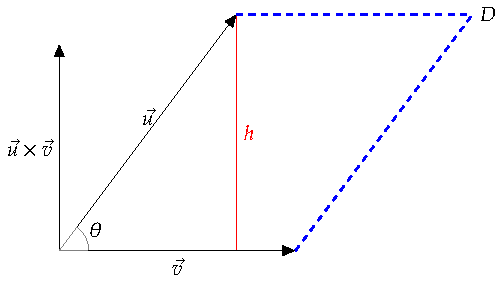
\includegraphics{area-paralelogramo.pdf}
  % \begin{tikzpicture}
  %   \coordinate (A) at (0,0);
  %   \coordinate (X) at (4,0);
  %   \coordinate (Y) at (3,4);
  %   \coordinate (W) at (0,3.5);

  %   \coordinate[label=right:$D$]  (D) at ($(X)+(Y)$);

  %   \draw[color=red] ($(A)!(Y)!(X)$) -- (Y) node[midway,right]{$h$};

  %   \draw[dashed,thick,color=blue] (X)--(D);
  %   \draw[dashed,thick,color=blue] (Y)--(D);
  %   \draw[->,>=triangle 45] (A) -- (X)
  %     node[midway,below]{$\vec{v}$};
  %   \draw[->,>=triangle 45] (A) -- (Y)
  %     node[midway,above]{$\vec{u}$};
  %   \draw[->,>=triangle 45] (A) -- (W)
  %     node[midway,left]{$\vec{u}\times\vec{v}$};


  %   % Mark the angle XAY
  %   \begin{scope}
  %     \path[clip] (A) -- (X) -- (Y);
  %     \fill[white, opacity=0.5, draw=black] (A) circle (5mm);
  %     \node at ($(A)+(30:7mm)$) {$\theta$};
  %   \end{scope}
  % \end{tikzpicture}
\end{figure}

A \'area $\mathcal{A}$ desse paralelogramo \'e dado Por
\[
  \mathcal{A} = bh.
\]
Neste caso $b = \norm{\vec{u}}$ e $h = \norm{\vec{v}}\sin\theta$. Logo
\[
  \mathcal{A} = \norm{\vec{u}}\norm{\vec{v}}\sin\theta = \norm{\vec{u}\times\vec{v}}.
\]
Portanto o vetor $\vec{u}\times\vec{v}$ \'e tal que seu m\'odulo \'e numericamente igual \`a \'area do paralelogramo definido por $\vec{u}$ e $\vec{v}$.
\begin{exemplo}
  Calcule a \'area do tri\^angulo de v\'ertices $A(3,2,0)$, $B(0,4,3)$ e $C(1,0,2)$.
  \begin{solucao}
    Note que a \'area do tri\^angulo \'e metade da \'area do paralelogramo. Assim seja
    \begin{align*}
      \vec{u} = \vec{CA} = (2,2,-2)\\
      \vec{v} = \vec{CB} = (-1,4,1)
    \end{align*}
    da{\'\i} a \'area do tri\^angulo ser\'a
    \[
      \mathcal{A} = \dfrac{\norm{\vec{u}\times\vec{v}}}{2}
    \]
    e como $\vec{u}\times\vec{v} = (10,0,10)$ temos $\mathcal{A} = 5\sqrt{2}$.
  \end{solucao}
\end{exemplo}
% subsection produto_vetorial (end)

\subsection{Produto Misto} % (fold)
\label{sub:produto_misto}

Sejam $\vec{u}$ e $\vec{v}$ vetores de $\real^3$. Como $\vec{u}\times\vec{v}$ \'e um vetor de $\real^3$ podemos calcular seu produto interno com qualquer outro vetor $\vec{w}$ de $\real^3$. O n\'umero real
\begin{equation}
  \langle\vec{u}\times\vec{v}, \vec{w}\rangle
\end{equation}
\'e chamado de \textbf{produto misto} dos vetores $\vec{u}$, $\vec{v}$ e $\vec{w}$.\index{Vetores no Espa\c{c}o!Produto Misto} Se $\vec{u} = (a_1,b_1,c_1)$, $\vec{v} =(a_2,b_2,c_2)$ e $\vec{w} = (a_3,b_3,c_3)$ temos
\begin{align*}
  \langle\vec{u}\times\vec{v}, \vec{w}\rangle &= \langle(b_1c_2 - c_2b_1,a_2c_1 - a_1c_2, a_1b_2 - a_2b_1), (a_3, b_3, c_3)\rangle \\ &= (b_1c_2 - b_2c_1)a_3 + (a_2c_1 - a_1c_2)b_2 + (a_1b_2 - a_2b_1)c_3.
\end{align*}

Agora,
\begin{align*}
  \det \begin{pmatrix}
    a_1 & b_1 & c_1\\
    a_2 & b_2 & c_2\\
    a_3 & b_3 & c_3
  \end{pmatrix} & = (-1)^{3+1}a_3\det \begin{pmatrix}
    b_1 & c_1\\
    b_2 & c_2
  \end{pmatrix} \\ &+ (-1)^{3+2}b_3\det \begin{pmatrix}
    a_1 & c_1\\
    a_2 & c_2
  \end{pmatrix} + (-1)^{3+3}c_3\det \begin{pmatrix}
    a_1 & b_1\\
    a_2 & b_2
  \end{pmatrix}\\ &= a_3(b_1c_2 - c_1b_2) - b_3(a_1c_2 - a_2c_1) + c_3(a_1b_2 - a_2b_1).
\end{align*}

Portanto
\begin{equation}
  \langle\vec{u}\times\vec{v}, \vec{w}\rangle = \det \begin{pmatrix}
    a_1 & b_1 & c_1\\
    a_2 & b_2 & c_2\\
    a_3 & b_3 & c_3
  \end{pmatrix}.
\end{equation}

\begin{proposicao}
  Sejam $\vec{u}$, $\vec{v}$ e $\vec{w}$ vetores em $\real^3$. Ent\~ao
  \begin{enumerate}[label=({\alph*})]
    \item $\langle\vec{u}\times\vec{v}, \vec{w}\rangle = \langle\vec{v}\times\vec{w}, \vec{u}\rangle$
    \item $\langle\vec{u}\times\vec{v}, \vec{w}\rangle = \langle\vec{u}, \vec{v}\times\vec{w}\rangle$
  \end{enumerate}
\end{proposicao}
\begin{prova}
  Segue diretamente das propriedades de determinantes.
\end{prova}

Sejam $\vec{u}$, $\vec{v}$ e $\vec{w}$ vetores em $\real^3$. Considere o paralelep{\'\i}pedo definido por $\vec{u}$, $\vec{v}$ e $\vec{w}$:
\begin{figure}[!h]
  \centering
  \caption{Interpreta\c{c}\~ao geom\'etrica do produto misto}
  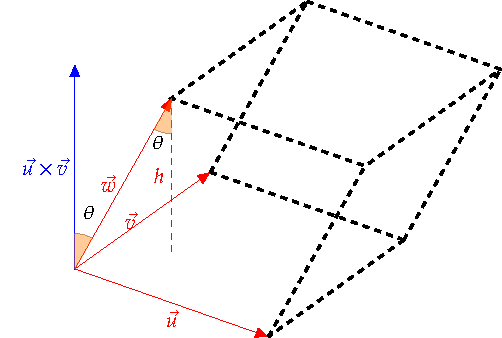
\includegraphics{volume-paralelepipedo.pdf}
  % \tdplotsetmaincoords{60}{125}
  % \begin{tikzpicture}
  %     [tdplot_main_coords,
  %       cube/.style={very thick,black},
  %       grid/.style={very thin,gray},
  %       axis/.style={->,blue,thick},scale=2]

  %   \coordinate (A) at (2,0,0);
  %   \coordinate (B) at (2,1,2);
  %   \coordinate (C) at (2,1,0.5);
  %   \coordinate (D) at (2,0,2);

  %   %draw the top and bottom of the cube
  %   \draw[dashed,cube] (0,0,0) -- (0,2,0);
  %   \draw[dashed,cube] (0,2,0) -- (2,2,0);
  %   \draw[->,>=triangle 45,color=red] (2,0,0) -- (2,2,0) node[midway,below]{$\vec{u}$};
  %   \draw[->,>=triangle 45,color=red] (2,0,0) -- (0,0,0) node[midway,left]{$\vec{v}$};
  %   %\draw[cube] (0,0,0) -- (0,2,0) -- (2,2,0) -- (2,0,0) -- cycle;
  %   \draw[dashed,cube] (0,1,2) -- (0,3,2) -- (2,3,2) -- (2,1,2) -- cycle;
  %   \draw[dashed,color=red] (2,1,0.5) -- (2,1,2) node[midway,left]{$h$};
  %   %draw the edges of the cube
  %   \draw[dashed,cube] (0,0,0) -- (0,1,2);
  %   \draw[dashed,cube] (0,2,0) -- (0,3,2);
  %   \draw[->,>=triangle 45,color=red] (2,0,0) -- (2,1,2) node[midway,left]{$\vec{w}$};
  %   \draw[->,>=triangle 45,color=blue] (2,0,0) -- (2,0,2) node[midway,left]{$\vec{u}\times\vec{v}$};
  %   \draw[dashed,cube] (2,2,0) -- (2,3,2);

  %   \tkzMarkAngle[fill=orange,size=0.3cm,opacity=.4](A,B,C);
  %   \draw ($(A)+(0.2,1,1.8)$) node[below,font=\small] {$\theta$};

  %   \tkzMarkAngle[fill=orange,size=0.3cm,opacity=.4](B,A,D);
  %   \draw ($(A)+(-0.2,0,0.6)$) node[below,font=\small] {$\theta$};
  % \end{tikzpicture}
\end{figure}

A altura $h$ \'e dada por
\begin{align*}
  h = \norm{\vec{w}}|\cos\theta| = \norm{\vec{w}}\dfrac{|\langle\vec{u}\times\vec{v}, \vec{w}\rangle|}{\norm{\vec{u}\times\vec{v}}\norm{\vec{w}}} = \dfrac{|\langle\vec{u}\times\vec{v}, \vec{w}\rangle|}{\norm{\vec{u}\times\vec{v}}}.
\end{align*}
O volume do paralelep{\'\i}pedo \'e
\[
  \mathcal{V} = \norm{\vec{u}\times\vec{v}}h
\]
da{\'\i}
\[
  \mathcal{V} = \norm{\vec{u}\times\vec{v}}\dfrac{|\langle\vec{u}\times\vec{v}, \vec{w}\rangle|}{\norm{\vec{u}\times\vec{v}}},
\]
isto \'e,
\begin{equation}
  \mathcal{V} = |\langle\vec{u}\times\vec{v}, \vec{w}\rangle|.
\end{equation}

\begin{exemplo}
  Os pontos $P(0,1,1)$, $Q(1,0,2)$, $R(1,-2,0)$ e $S(-2,2,-2)$ definem um paralelep{\'\i}pedo? Em caso afirmativo, qual o seu volume?
  \begin{solucao}
    Se os pontos $P$, $Q$, $R$ e $S$ definirem um paralelep{\'\i}pedo, seu volume dever\'a ser diferente de zero. Assim considere os vetores
    \begin{align*}
      \vec{u} = \vec{PQ} = (1,-1,1)\\
      \vec{v} = \vec{PR} = (1,-3,-1)\\
      \vec{w} = \vec{PS} = (-2,1,-3).
    \end{align*}
    Assim temos
    \begin{align*}
      \langle\vec{u}\times\vec{v}, \vec{w}\rangle = \det \begin{bmatrix}
        1 & -1 & 1\\
        1 & -3 & -1\\
        -2 & 1 & -3
      \end{bmatrix} = 0.
    \end{align*}
    Logo $P$, $Q$, $R$ e $S$ n\~ao definem um paralelep{\'\i}pedo.
  \end{solucao}
\end{exemplo}
% subsection produto_misto (end)

% chapter vetores_no_espaco (end)